\documentclass[preprint,12pt]{elsarticle}
% major revision and answer question (3 reviewers)
%Sunday, January 24⋅22:30 – 22:55
%Daily, until Jan 29, 2021

% mark in blue or red
\usepackage{xcolor}

\newenvironment{MyColorPar}[1]{%
    \leavevmode\color{#1}\ignorespaces%
}{%
}%

\usepackage{outlines}

%%% for abbreviations, or acronyms
\usepackage[automake, acronym, nopostdot]{glossaries} 
%\usepackage{glossary-inline}
%\newenvironment{abbreviation}
%\makeglossaries %https://tex.stackexchange.com/questions/110095/list-of-acronyms-is-not-displayed
\newacronym{fdr}{FDR}{false discovery rate}
\newacronym{hpa}{HPA}{the Human Protein Atlas}
\newacronym{hnscc}{HNSCC}{head and neck squamous cell carcinoma}
\newacronym{tcga}{TCGA}{the Cancer Genome Atlas}
\newacronym{tcpa}{TCPA}{the Cancer Proteome Atlas}
\newacronym{rna}{RNA}{ribonucleic acid}
\newacronym{rnaseq}{RNA-Seq}{RNA sequencing}
\newacronym{lncrna}{lncRNA}{long non-coding RNA}
%\newacronym{km}{KM}{Kaplan-Meier}
\newacronym{rppa}{RPPAs}{reverse-phase protein arrays}
\newacronym{rpma}{RPMA}{reverse-phase protein lysate microarray}

\newacronym{mmp}{MMP}{matrix metalloproteinase}
 %DKK1, CAMK2N1, STC2, PGK1, SURF4, USP10, NDFIP1, FOXA2, STIP1, and DKC1
 %ZNF557, ZNF266, IL19, MYO1H, FCGBP, LOC148709, EVPLL, PNMA5, KIAA1683, and NPB

\newacronym{DKK1}{DKK1}{dickkopf WNT signaling pathway inhibitor 1} 
\newacronym{CAMK2N1}{CAMK2N1}{calcium/calmodulin dependent protein kinase II inhibitor 1} 
\newacronym{STC2}{STC2}{stanniocalcin 2} 
\newacronym{PGK1}{PGK1}{phosphoglycerate kinase 1} 
\newacronym{SURF4}{SURF4}{surfeit 4} 
\newacronym{USP10}{USP10}{ubiquitin specific peptidase 10} 
\newacronym{NEDD4}{NEDD4}{neural precursor cell expressed, developmentally down-regulated 4}
\newacronym{NDFIP1}{NDFIP1}{NEDD4 family interacting protein 1} 
\newacronym{FOXA2}{FOXA2}{forkhead box A2} 
\newacronym{STIP1}{STIP1}{stress-induced-phosphoprotein 1} 
\newacronym{DKC1}{DKC1}{dyskeratosis congenita 1, dyskerin} 

\newacronym{ZNF557}{ZNF557}{zinc finger protein 557} 
\newacronym{ZNF266}{ZNF266}{zinc finger protein 266} 
\newacronym{IL19}{IL19}{interleukin 19} 
\newacronym{MYO1H}{MYO1H}{myosin 1H} 
\newacronym{FCGBP}{FCGBP}{Fc fragment of IgG binding protein} 
\newacronym{LOC148709}{LOC148709}{LncRNA LOC148709} 
\newacronym{EVPLL}{EVPLL}{envoplakin-like protein} 
\newacronym{PNMA5}{PNMA5}{paraneoplastic antigen like 5} 
%\newacronym{KIAA1683}{KIAA1683}{IQCN, IQ Motif Containing N} 
\newacronym{IQCN}{IQCN}{IQ motif containing N} % previous name KIAA1683
% "IQ" refers to the first two amino acids of the motif: isoleucine (commonly) and glutamine (invariably)
\newacronym{NPB}{NPB}{neuropeptide B} 

 \newacronym{rt}{RT}{radiation therapy}
 \newacronym{nccn}{NCCN}{National Comprehensive Cancer Network}
 \newacronym{hif}{HIF}{hypoxia-inducible factor}
 \newacronym{egfr}{EGFR}{epidermal growth factor receptor}
 \newacronym{ras}{RAS}{rat sarcoma}
 \newacronym{hras}{HRAS}{Harvey rat sarcoma viral oncoprotein}
 \newacronym{erk}{ERK}{extracellular signal-regulated kinases}
 \newacronym{us}{US}{United States}
 \newacronym{fda}{FDA}{Food and Drug Administration}
 \newacronym{tpf}{Tax-PF}{docetaxel, cisplatin, and 5-fluorouracil}
 \newacronym{tki}{TKI}{tyrosine kinase inhibitor}
 \newacronym{her}{HER}{human epidermal growth factor receptor}
 \newacronym{ici}{ICI}{immune-checkpoint inhibitor}
 \newacronym{ctla4}{CTLA-4}{cytotoxic T lymphocyte antigen 4}
 \newacronym{pd1}{PD-1}{programmed death 1}
 \newacronym{pdl1}{PD-L1}{programmed death ligand 1}
 \newacronym{tim3}{TIM-3}{T-cell immunoglobulin mucin protein 3}
 \newacronym{lag3}{LAG-3}{lymphocyte activation gene 3}
 \newacronym{ifng}{IFN-$\gamma$}{interferon gamma}
 \newacronym{tigit}{TIGIT}{T cell immunoglobin and immunoreceptor tyrosine-based inhibitory motif}
 \newacronym{gitr}{GITR}{glucocorticoid-induced tumor necrosis factor receptor}
 \newacronym{vista}{VISTA}{V-domain Ig suppressor of T-cell activation}
 \newacronym{tmsb4x}{TMSB4X}{thymosin beta-4 X-linked}
 \newacronym{emt}{EMT}{epithelial-mesenchymal-transition}
 \newacronym{gdc}{GDC}{Genomic Data Commons}
 \newacronym{nci}{NCI}{the National Cancer Institute}
 \newacronym{gdac}{GDAC}{Genome Data Analysis Center}
 \newacronym{rest}{REST}{Representational State Transfer} 
 \newacronym{api}{API}{Application Programmable Interface}
\newacronym{grch38}{GRCh38}{Genome Reference Consortium Homo sapiens genome assembly 38}
\newacronym{fpkm}{FPKM}{Fragments per kilobase per million reads mapped}
\newacronym{rsem}{RSEM}{RNA-Seq by Expectation-Maximization}
\newacronym{slca}{SLC35E2A}{solute carrier family 35 member E2A}
\newacronym{slcb}{SLC35E2B}{solute carrier family 35 member E2B}
\newacronym{cde}{CDE}{Common Data Element}
\newacronym{id}{ID}{identification}
\newacronym{ajcc}{AJCC}{the American Joint Committee on Cancer}
\newacronym{uicc}{UICC}{he Union for International Cancer Control}
\newacronym{tnm}{TNM}{the tumor size (T), cervical lymph node metastases (N), and distal metastasis status (M)}
\newacronym{ci95}{95\% CI}{95\% confidence interval}
\newacronym{os}{OS}{overall survival}
\newacronym{hr}{HR}{hazard ratio}
\newacronym{hpv}{HPV}{human papillomavirus}
\newacronym{ene}{ENE}{extra-nodal extension}
\newacronym{lvsi}{LVSI}{lymph-vascular space invasion}
\newacronym{pni}{PNI}{perineural invasion}
\newacronym{doi}{DOI}{depth of invasion}
\newacronym{lnd}{LND}{lymph node density}
\newacronym{wpoi5}{WPOI-5}{worst pattern of invasion score 5}
\newacronym{glut4}{GLUT4}{glucose transporters 4}
\newacronym{slc2a4}{SLC2A4}{solute carrier family 2 member A4}
\newacronym{trim24}{TRIM24}{tripartite motif-containing 24}
\newacronym{til}{TIL}{tumor-infiltrating lymphocytes}
\newacronym{tmb}{TMB}{tumor mutational burden}



%==================
\begin{document}

\section{Revision cover letter (cancers-1082127)} % 2021/01/25
%其實直接 online 填寫即可
%Please provide a cover letter to explain point-by-point the details of the revisions [changes 摘要即可 from the rebuttal]  in the manuscript
 

%Assistant Editor
%E-Mail: aubree.zhu@mdpi.com
%MDPI Branch Office, Tianjin
Assistant Editor of Cancers%\newline

Jan 29, 2021

Dear Dr. Aubree Zhu:

Enclosed, please find our revised manuscript (cancers-1082127) entitled "A Global Genome-wide Scan with Optimal Cutoff Mining for Emerging Biomarkers in Head and Neck Squamous Cell Carcinoma" by Chi et al., which we wish to be considered for publishing as a research article in Cancers. We greatly appreciate your time in serving as the editor handling this manuscript and also thank the reviewers for their critical comments and suggestions on our manuscript.

We have since performed additional analysis, experiment and revised the manuscript accordingly to address their critical comments and suggestions in a point-by-point manner, 
%

According to the editor's comments, we have the manuscript checked for English grammar and reformat Table 1 by rotating 90 degrees to portrait mode. %(Table 1 轉正)

%

We wish our revised manuscript could be satisfied and accepted for publication in Cancers. Thanks very much for the kind helps and the reviewers' critical comments.

Kind regards,

Yu-Chuan (Jack) Li, M.D., Ph.D.

Graduate Institute of Biomedical Informatics, 

College of Medical Science and Technology,

Taipei Medical University,

Taipei, Taiwan

%2) [cancers-1082127_main_redMarked] 自動化 by latex:
%"Track Changes" function in latex => by latexdiff
%Some options, taken from the documentation, include:
%UNDERLINE—added text is wavy-underlined and blue, discarded text is struck out and red;
%CTRADITIONAL—added text is blue and set in sans-serif, and a red footnote is created for each discarded piece of text;
%TRADITIONAL—like CTRADITIONAL but without the use of colour;
%CFONT—added text is blue and set in sans-serif, and discarded text is red and very small size;
%FONTSTRIKE—added text is set in sans-serif, discarded text small and struck out;
%CHANGEBAR—added text is blue, and discarded text is red. Additionally, the changed text is marked with a bar in the margin.
%https://www.overleaf.com/learn/latex/Articles/Using_Latexdiff_For_Marking_Changes_To_Tex_Documents

\pagebreak

\section{rebuttal} % Response2Referees
We greatly appreciate the reviewers for their helpful suggestions and critical comments on our manuscript. The detailed point-by-point reply to the reviewer’s comments are as follows (marked as \textcolor{blue}{blue}). 
And the revised portions in the manuscript are indicated in \textcolor{red}{red}.

%Reviewer #1(Technical Comments to the Author):
%   The ms investigates an interesting and timely topic. However, the discovery cohort involves a small sample size and throughout the analysis, the issue of correcting the obtained p-values for multiple comparisons is not addressed. Hence, the evidence for zooming into TMSB4X is not convincing.

%\section{Responses to Reviewers' comments}
% our responses to the reviewers' comments.
%***Response to reviewer's comments: [藍色字]

Comments from the reviewer \#1:

Comments and Suggestions for Authors
The authors have described the effectiveness of RNA sequencing as a tool for exploring prognostic factors; they have also performed a large-scale analysis using the TCGA cohort, which is a very attractive analysis method. I have a few minor questions.

This is an attractive analysis method and I would like to know more details.

\subsection*{1-1}
It is generally known that high expression of EGFR is a poor prognostic factor in head and neck cancers, however, why is it that RNA sequencing does not identify RNA coding for EGFR as a poor prognostic factor?

\begin{MyColorPar}{blue}
Answer

We appreciate the reviewer for the critical comments and thank for his/her agreement of our analysis using the TCGA cohort.
%[我的 candidate 中為什麼沒有 EGFR];  
In our analysis, the \acrshort{egfr} is ranked at 5707 from 20500 protein-coding genes %5708-1
by Kaplan-Meier estimate with the log-rank test P-value as 0.0495. The \acrshort{egfr} is identified as one of those poor prognostic factors as well. %However, it is far from the top 20 candidates.
(please see https://github.com/texchi2/\linebreak
pvalueTex/blob/master/HNSCC\_OS\_marginS\_6429.csv for reference, the table was ranked by FDR P-value)

% transforming growth factor- (TGF-α) 
% epidermal growth factor receptor (EGFR)
As in our manuscript mentioned, 
In a multivariate analysis, tumor site, tumor level of \acrshort{egfr}, and tumor level of TGF-$\alpha$ (\acrshort{egfr} ligand) were statistically significant predictors of disease-free survival of \acrshort{hnscc} patients\cite{Rusch1996}\cite{Grandis1998}.
Since that breakthrough discovery and validation, the \acrshort{egfr} monoclonal antibody (cetuximab)\cite{Bonner2006a} and \acrshort{egfr} \acrshort{tki} (such as gefitinib, erlotinib, osimertinib) were developed to treat advanced \acrshort{hnscc}. Although 90\% of \acrshort{hnscc} has overexpression of \acrshort{egfr}, cetuximab has only 10\% to 20\% response rate on those patients\cite{Johnson2020}. So far, cetuximab is still the only drug of choice with proven efficacy, which targeted the selected \acrshort{hnscc} patients\cite{Taberna2019}.
%citing the line number and exact change, marked in \textcolor{red}{Red from page 6 (line 16) to page 7 (line 17)}
Thus, we wish the further validations of our meaningful hypotheses of candidate to explore more useful drug of choice in the treatment of \acrshort{hnscc} patients.
% a list from literature review, 留 下少於  50 articles mentioned candidates
%HNSCC_survivalAnalysis_marginS_EGFR.Rda
%HNSCC_survivalAnalysis_marginS_EGFR.xlsx
%https://github.com/texchi2/pvalueTex/blob/master/file20500_list.txt
%analysis_export.R to generate https://github.com/texchi2/pvalueTex/blob/master/HNSCC_OS_marginS_6429.csv
\end{MyColorPar}


\subsection*{1-2}
DNA alteration (mutation/amplification) is also an influential prognostic factor, but I would like to know if DNA alteration is considered in this analysis.
%[如果加入 DNA alteration 又會如何? 不佳; 選擇 mRNA 的原因是? interpretability and drugable: EGFR]

\begin{MyColorPar}{blue}
Answer

We appreciate the reviewer for reminding the importance of DNA alteration in survival analysis.
Those different types of omics data measured for the same patients (called multi-omics data) are currently under investigation across several disciplines such as genomics (i.e. DNA mutation/amplification, single nucleotide polymorphisms), %copy number variation), 
epigenomics, transcriptomics (i.e. RNA expression), proteomics, metabolomics and microbiomics.
The usefulness of multi-omics data for the prediction of HNSCC outcome is expected.
%such as the (censored) survival time.
Moritz Herrmann et al.(2020) observed that using multi-omics and survival data can slightly improve the performance of prediction methods for particular datasets, such as TCGA HNSCC\cite{Herrmann2020}.
%It is limited that the utility of multi-omics data for prediction purposes in the considered TCGA studies\cite{Herrmann2020}.
%18 cancer datasets from The Cancer Genome Atlas (TCGA) 
According to their study, %the multi-omics structure have a slightly better prediction performance than naive (0.562 vs.	0.557 ) with favoring clinical variables leads to better prediction results for HNSCC. %likelihood-based boosting (CoxBoost and CoxBoost favoring)
% Exemplary t-tests comparing blockForest with CoxBoost favoring and the Clinical only model showed no significant differences in performance. 
% blockForest also offers the possibility of favoring clinical covariates using the argument always.select.block of the blockfor function
%Last but not the least, multi-omics data are structured: the variables are partitioned into (non overlapping) groups. 
% ***
the survival analysis of TCGA HNSCC dataset by blockForest method (with multi-omics and clinical variables) has a similar prediction performance than that by Cox's model (with clinical variables alone). %from The Cancer Genome Atlas (TCGA) 
They also reported the performance C-index as 0.582 [CI: 0.554, 0.610] in blockForest method and 0.554 [CI: 0.519, 0.588] in Cox's model\cite{Herrmann2020}.

% 小心光茫太甚  Well-established prognostic clinical variables: prioritize
% the number of variables in the group of variables of TCGA HNSCC dataset:
% 11 clinical variables, 57964 CNV variables, 17248 mutation variables and 21520 RNA expression variables.
%*** Taking this structure into account can protect the predictive information that transcriptomics (e.x. RNA-Seq) or low-dimensional clinical variables might get lost within the huge amount of genomics (e.x. DNA mutation/amplification, copy number variation) data\cite{Boulesteix2011}\cite{Herrmann2020}.
DNA amplification will usually be one of the causes to overexpress the gene.
Moreover, transcriptomics study is helpful in drug discovery. For example, the overexpressed gene is possible to be a drug-targetable candidate\cite{Park2015}. After thoughtful validation in vitro/in vivo then pathway study, the EGFR inhibitory leads were constructed by antibody design or chemical compound screening\cite{Mahajan2016}. %比較容易研發 clinical and transcriptomics by ssurvival::survfit and urvival::coxph
% the selection of clinicalfeatures by domain knowledge and studies where HNSCC was under investigation.
The discovery of EGFR inhibitors\cite{Bonner2006a} for HNSCC therapy will encourage research community to conduct the survival analysis under abnormality in gene expression.

% *** it needs deep learning, but less interpretability (yet under development\cite{Chaudhary2018}) (DNA+RNA and clinical dataset => multi-omics cancer study)
%high dimensional multi-omics analysis by deep learning 
%It may be beneficial to include these different data types in models predicting outcomes, such as the survival time of patients. Until recently, only data from a single omics type were used to build such prediction models, with or without the inclusion of standard clinical data [2]. In recent years, however, the increasing availability of different types of omics data measured for the same patients (called multi-omics data from now on) has led to their combined use for building outcome prediction models. An important characteristic of multi-omics data is the high-dimensionality of the datasets, which frequently have more than 10 000 or even 100 000 variables. This places particular demands on the methods used to build prediction models: they must be able to handle data where the number of variables by far exceeds the number of observations. Moreover, practitioners often prefer sparse and interpretable models containing only a few variables [3]. Last but not the least, multi-omics data are structured: the variables are partitioned into (nonoverlapping) groups. This structure may be taken into account when building prediction models.
%Citation: https://academic.oup.com/bib/advance-article/doi/10.1093/bib/bbaa167/5895463
%特別的 algorithm 
%however, interpretation and practical application of the model to the prediction of independent data are easier with regression-based methods yielding coefficients that reflect the effects of variables on the outcome than with machine learning algorithms [8].
%Multi-omics data, that is, datasets containing different types of high-dimensional molecular variables; they must be able to handle data where the number of variables by far exceeds the number of observations.
%https://www.ncbi.nlm.nih.gov/pmc/articles/PMC6419526/
%Deep learning
%SALMON (Survival Analysis Learning with Multi-Omics Neural Networks)

%\cite{Lawrence2015a} TCGA HNSCC %的第一篇文章已經分析過 DNA mutation of HNSCC
%Comprehensive genomic characterization of head and neck squamous cell carcinomas. Nature, 517(7536), 576–582. 
%https://www.cancer.gov/about-nci/organization/ccg/research/structural-genomics/tcga/publications
%=> HNSCC marker paper\cite{Lawrence2015a}

%The presence of widespread genomic instability in HNSCC, such as cytogenetic aberrations, allelic imbalance/loss of heterozygosity, and microsatellite instability (MSI), suggests that there is an imperfection in the host DNA repair machinery. Genomic instability with progressive accumulation of detrimental genetic alterations appears to be dependent upon a circuitous interaction between the environmental genotoxic insults and the host DNA repair machinery, the functional integrity of which is governed by the proper cell cycle control and host DNA repair capacity. Genomics allows the identification of possibly relevant variants, such as single nucleotide polymorphisms (SNPs), copy number variation (CNV), mutations and translocations => %https://cancersheadneck.biomedcentral.com/articles/10.1186/s41199-020-0047-y
%DNA mutation: copy number burden (CNB) and tumor mutation burden (TMB) are important for predicting tumor progression (Marshall et al., 2017; Thomas et al., 2018)
% *** The Landscape of Somatic Copy Number Alterations in Head and Neck Squamous Cell Carcinoma, 2020. => 18 GEO dataset (873 patients from GEO) + TCGA: chromothripsis 6\%\cite{Yang2020}
%metaanalysis of NCBI GEO database (https://www.ncbi.nlm.nih.gov/geo/). We integrated the following datasets: TCGA-HNSCC, GSE11938, GSE20306, GSE20939, GSE23831, GSE25103, GSE31984, GSE33229, GSE33983, GSE34507, GSE36790, GSE39367, GSE40777,GSE47443, GSE51265, GSE57201, GSE66136, GSE68717, and GSE85514.

%TMB: To calculate TMB, you need to know the total size of the region sequenced. If data is from exome sequencing, you would find the size of the exome capture, and divide total mutations (or non-synonymous only depending on strategy), by that size (e.g. ~45MB) to get SNV/MB ratio.
%tumor mutational burden-high (TMB-H) [≥10 mutations/megabase (mut/Mb)] in solid tumors (criteria for pembrolizumab)
%Identification of Genomic Predictors for Treatment Response to Cancer Immunotherapy Using Omics Data Analysis (Yu-Chao Wang)
%=> ICIs criteria <- TMB <- DDR DNA repair gene
\end{MyColorPar}
\pagebreak
%======

Comments from the reviewer \#2

How representative is the TCGA database for HNSCC?

Can be the found positive and negative prognostic genes underlined by comparable studies using other databases than TCGA?

Could the authors summarize the elements of the workflow that could be used on any database independently from TCGA?

Please shortly explain the TCGA database in the Introduction and summarize the advantages of its use.

%[找出其他 database cohort 的比較]
\subsection*{2-1}
How representative is the TCGA database for HNSCC?

\begin{MyColorPar}{blue}
Answer

We appreciate the reviewer for the question giving an opportunity to discuss TCGA in detail.\\
To the best of our knowledge, TCGA "HNSC"(they coded) is the only single and largest collection of whole-genome sequencing and clinical survival dataset in the field of HNSCC research so far.
When we queried from the Embase database using the MESH words "HNSCC AND TCGA", a simple statistics shows total 12,636 research articles/conference abstracts for HNSCC from 2008 to 2021, since the first TCGA article was published on 2008\cite{McLendon2008} by TCGA research network.
Thereafter, there are 18,082 cross-cancer type articles which were produced using TCGA database. The 778 publications (Figure \ref{figure:fig_embase}, b. 778) among them were focused on HNSCC research. Those occupied about 18\% of HNSCC research articles with genetic-related topics during the same time period. Thus, about 60 TCGA HNSCC articles were published worldwide per year since 2008. %\ref{figure:fig_embase}
\begin{figure}
\raggedleft
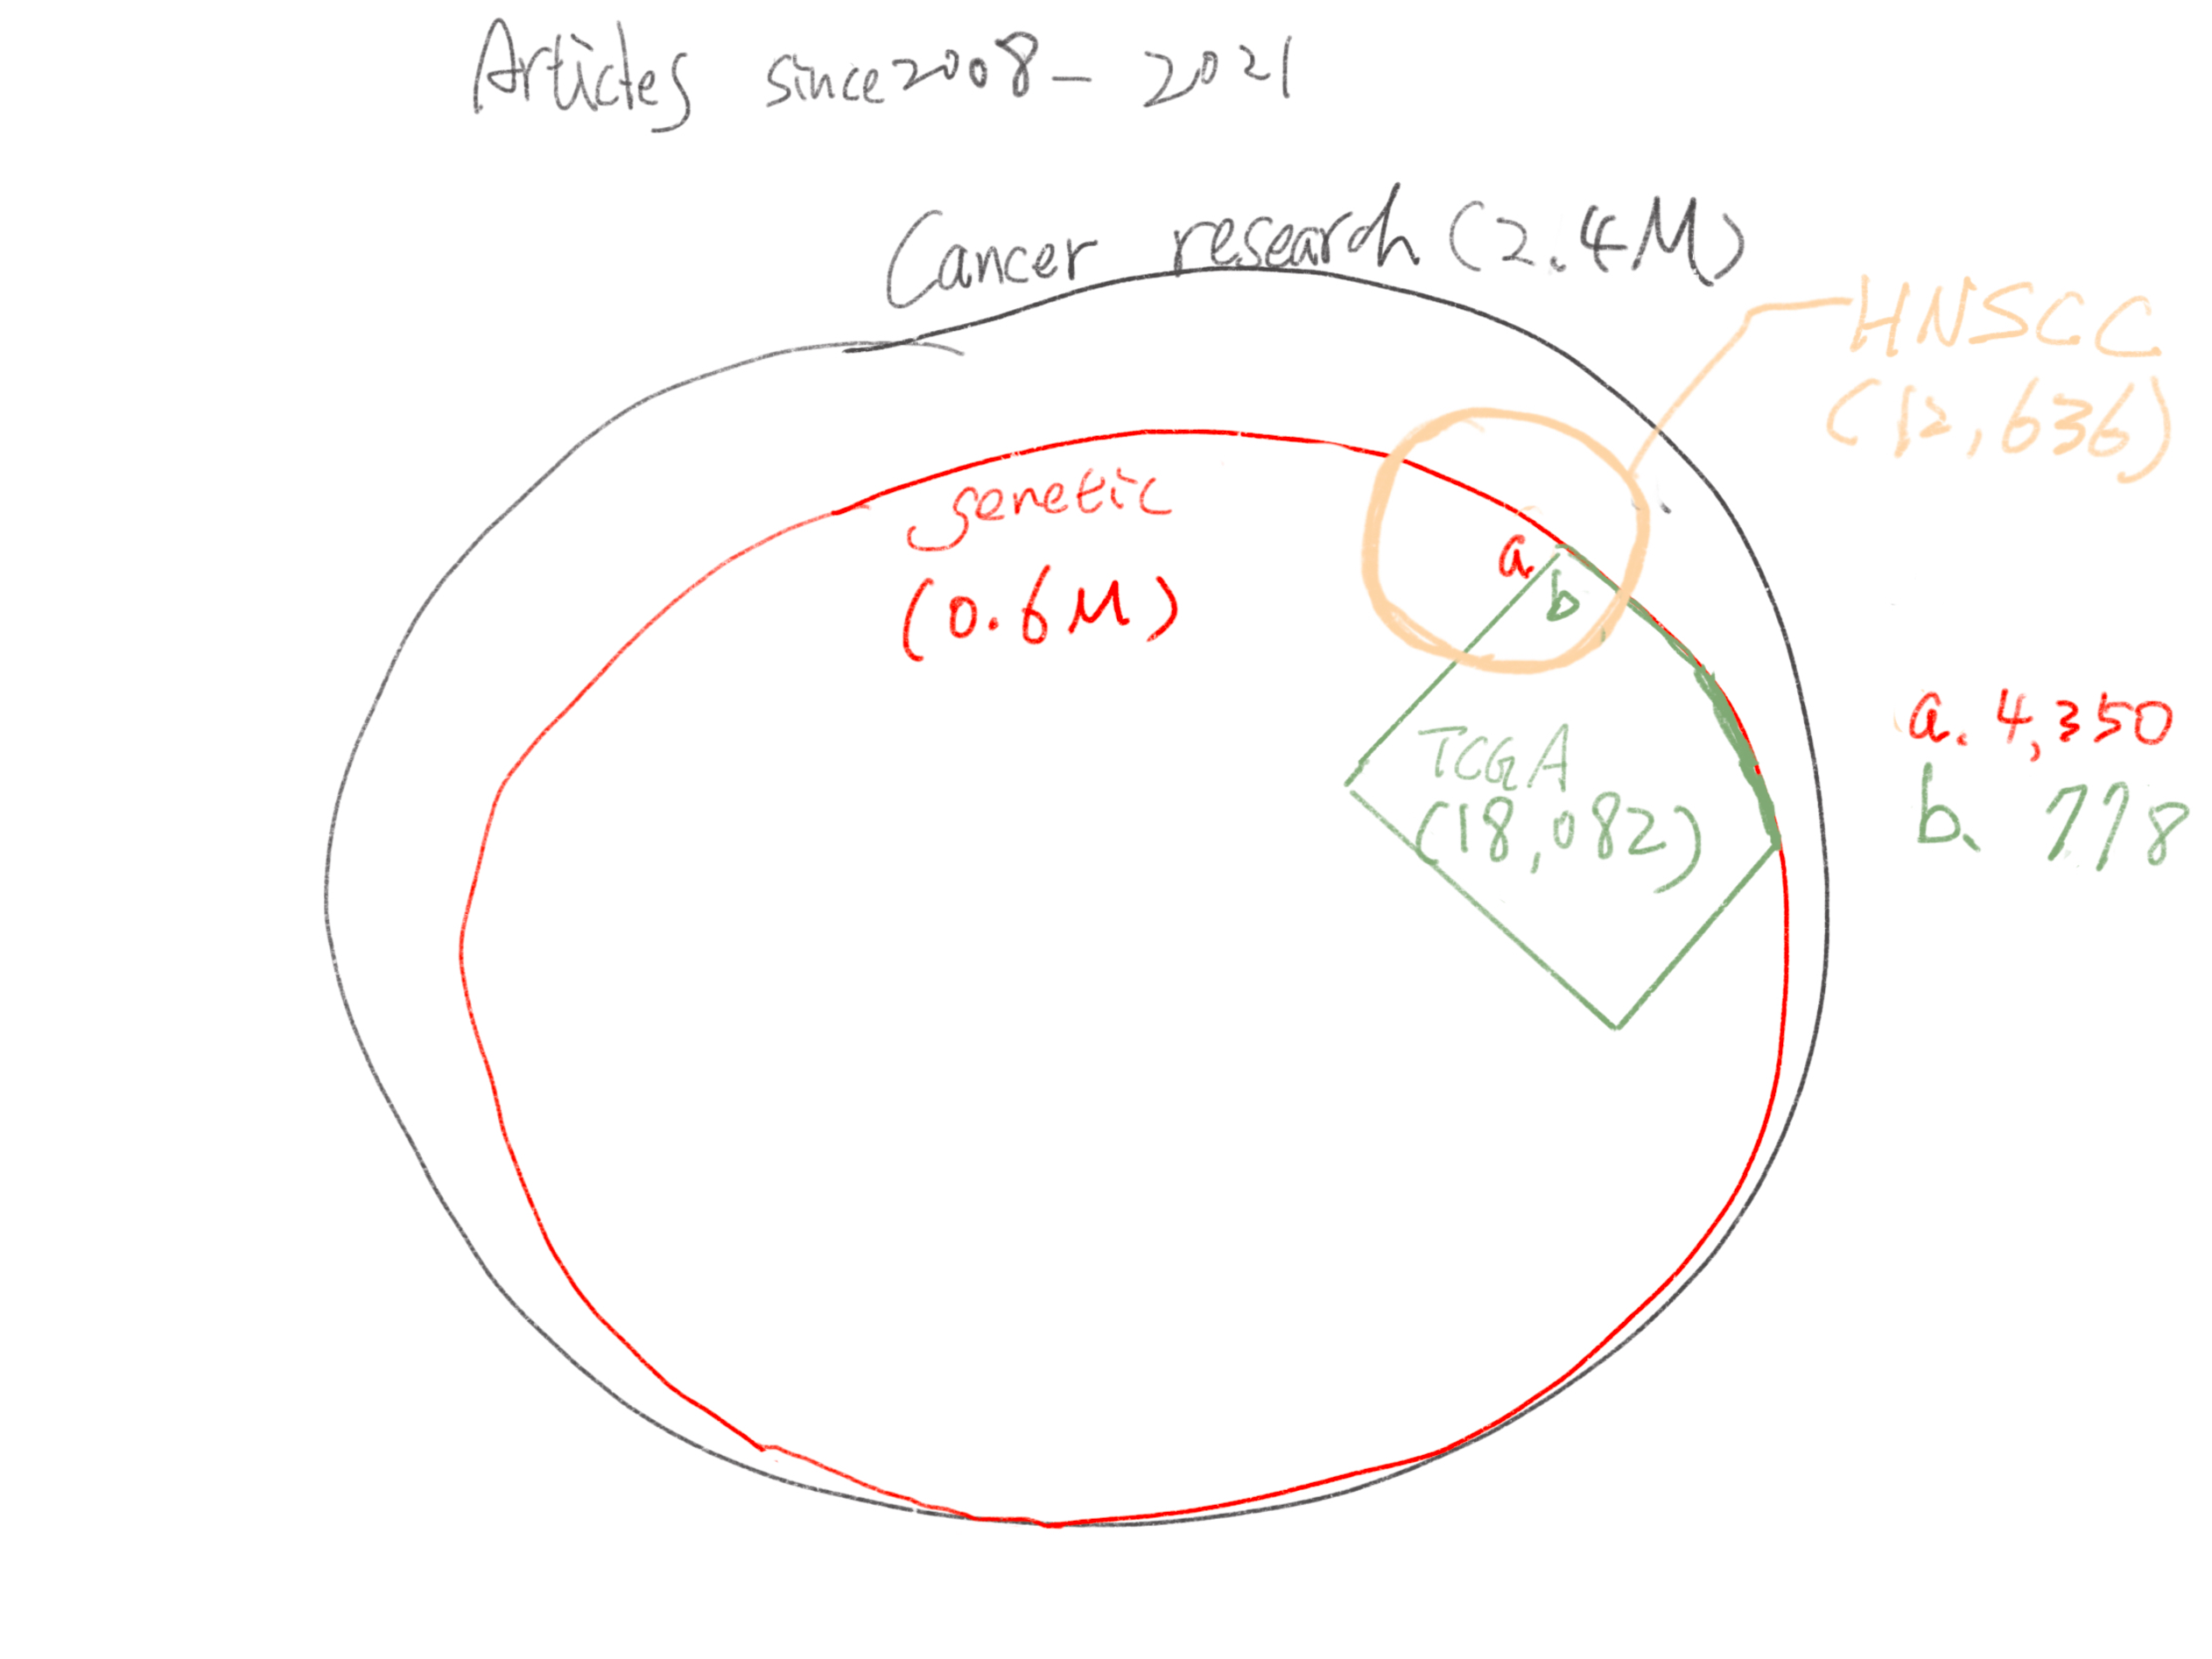
\includegraphics[width=14cm]{Answer_2-1.pdf}
\caption{Cancer research articles published from 2008 to 2021. Total: 2.4 million; genetic related: 0.6 million; HNSCC research: 12,636.}
\label{figure:fig_embase}
\end{figure}
\clearpage
%778/4350 = 17.9\% using TCGA data
%There is 374 genes in the oral cancer gene database of Indian HNSCC; http://www.bioinformation.net/006/97320630006169.pdf
%http://www.actrec.gov.in/OCDB/index.htm

Despite of other databases carrying HNSCC genomics and clinical data we found, such as MSKCC (151 cases), Broad (74 cases), Johns Hopkins (32 cases), MD Anderson (40 cases), and NCBI Gene Expression Omnibus (GEO) datasets (e.x. GSE2837, 40 cases; GSE6631, 22 cases; GSE31056, 23 cases)\cite{Cerami2012b}\cite{Gao2013a}. However,  MSKCC, Broad and Johns Hopkins databases were processed the whole-exome sequencing instead of whole-genome sequencing in TCGA database.

There is several useful web-tools for survival analysis, such as cBioportal\cite{Cerami2012b}\cite{Gao2013a}, KM-Plotter\cite{Gyorffy2010},  SurvExpress\cite{Aguirre-Gamboa2013}, and UALCAN (available at http://ualcan\\.path.uab.edu/)\cite{Chandrashekar2017a}. According to the citing articles\cite{Wu2020} and their online documents, the back-end databases of those web-tools were collected from TCGA, the European Genome-phenome Archive (EGA)\cite{Lappalainen2015} and NCBI GEO datasets (available at https://www.ncbi.nlm.nih.gov/gds). Furthermore, almost all of their survival data came from TCGA database.
%GEO (few survival features, less than 100 participate in each GSE dataset)
%GSE31056, GSE2837 (Prognoscan)
%there is survival feature: A total of 44 patients (22 HNSCC samples and 22 normal samples) were obtained from GSE6631
%有文章為證1. Lawrence, M. S. et al. Comprehensive genomic characterization of head and neck squamous cell carcinomas. Nature 517, 576–582 (2015).\cite{Lawrence2015a}
%datasets for each cancer type that include exactly the same prediction and outcome variables and consider comparable target populations. Currently, such data is simply not available.

Conclusion: TCGA database is representative for HNSCC.

\end{MyColorPar}

\subsection*{2-2}
Can be the found positive and negative prognostic genes underlined by comparable studies using other databases than TCGA?

\begin{MyColorPar}{blue}
Answer

We appreciate the reviewer for the critical comment.
We analysed GSE2837 dataset (NCBI GEO database\cite{Chung2006}, HNSCC cohort has 28 participants) from online tools: PrognoScan (availalbe at http://dna00.bio.kyutech.ac.jp/PrognoScan/)\cite{Mizuno2009a}.
%??MD Anderson (40 cases) SurvNet: https://bioinformatics.mdanderson.org/SurvNet/
%https://www.ncbi.nlm.nih.gov/geo/query/acc.cgi?acc=GSE2837 \cite{Chung2006}
The GSE2837 carries
% VUMC, VAMC, UTMDACC (1992-2005)
relapse free survival (RFS) data, instead of overall survival in TCGA dataset,
and microarray gene expression (by Affymetrix X3P chips U133\_X3P).
The survival significance (Kaplan Meier P-value) is in the following probes of 10 genes:\\
1) poor prognosis: CAMK2N1 (0.048214), PGK1 (0.009978), SURF4 (0.023127), USP10 (0.017768), NDFIP1 (0.022758), FOXA2 (0.001587); % FOXA2 (0.038125)
2) better prognosis: IL19 (0.049731), FCGBP (0.005658), KIAA1683 (IQCN, 0.005886), NPB (0.014177);
%17 out of 20 candidates
%?DKK1 (0.253635), 
Please see Figure \ref{figure:fig_GSE2837}.
Nevertheless, PrognoScan has group separation cut by a skewed manner, and the GSE2837 has far less participants than TCGA cohort.
%DKK1, CAMK2N1, STC2, PGK1, SURF4, USP10, NDFIP1, FOXA2, STIP1, DKC1;
%ZNF557, ZNF266, IL19, MYO1H, FCGBP, LOC148709, EVPLL, PNMA5, KIAA1683 (IQCN), NPB
%Those 11 genes achieve similar positive and negative prognostic effect comparable with our proposed candidate genes. 
The 10 out of 20 positive and negative prognostic genes underlined is confirmed by comparable studies using GSE2837 dataset other than TCGA cohort.

\begin{figure}
\raggedleft
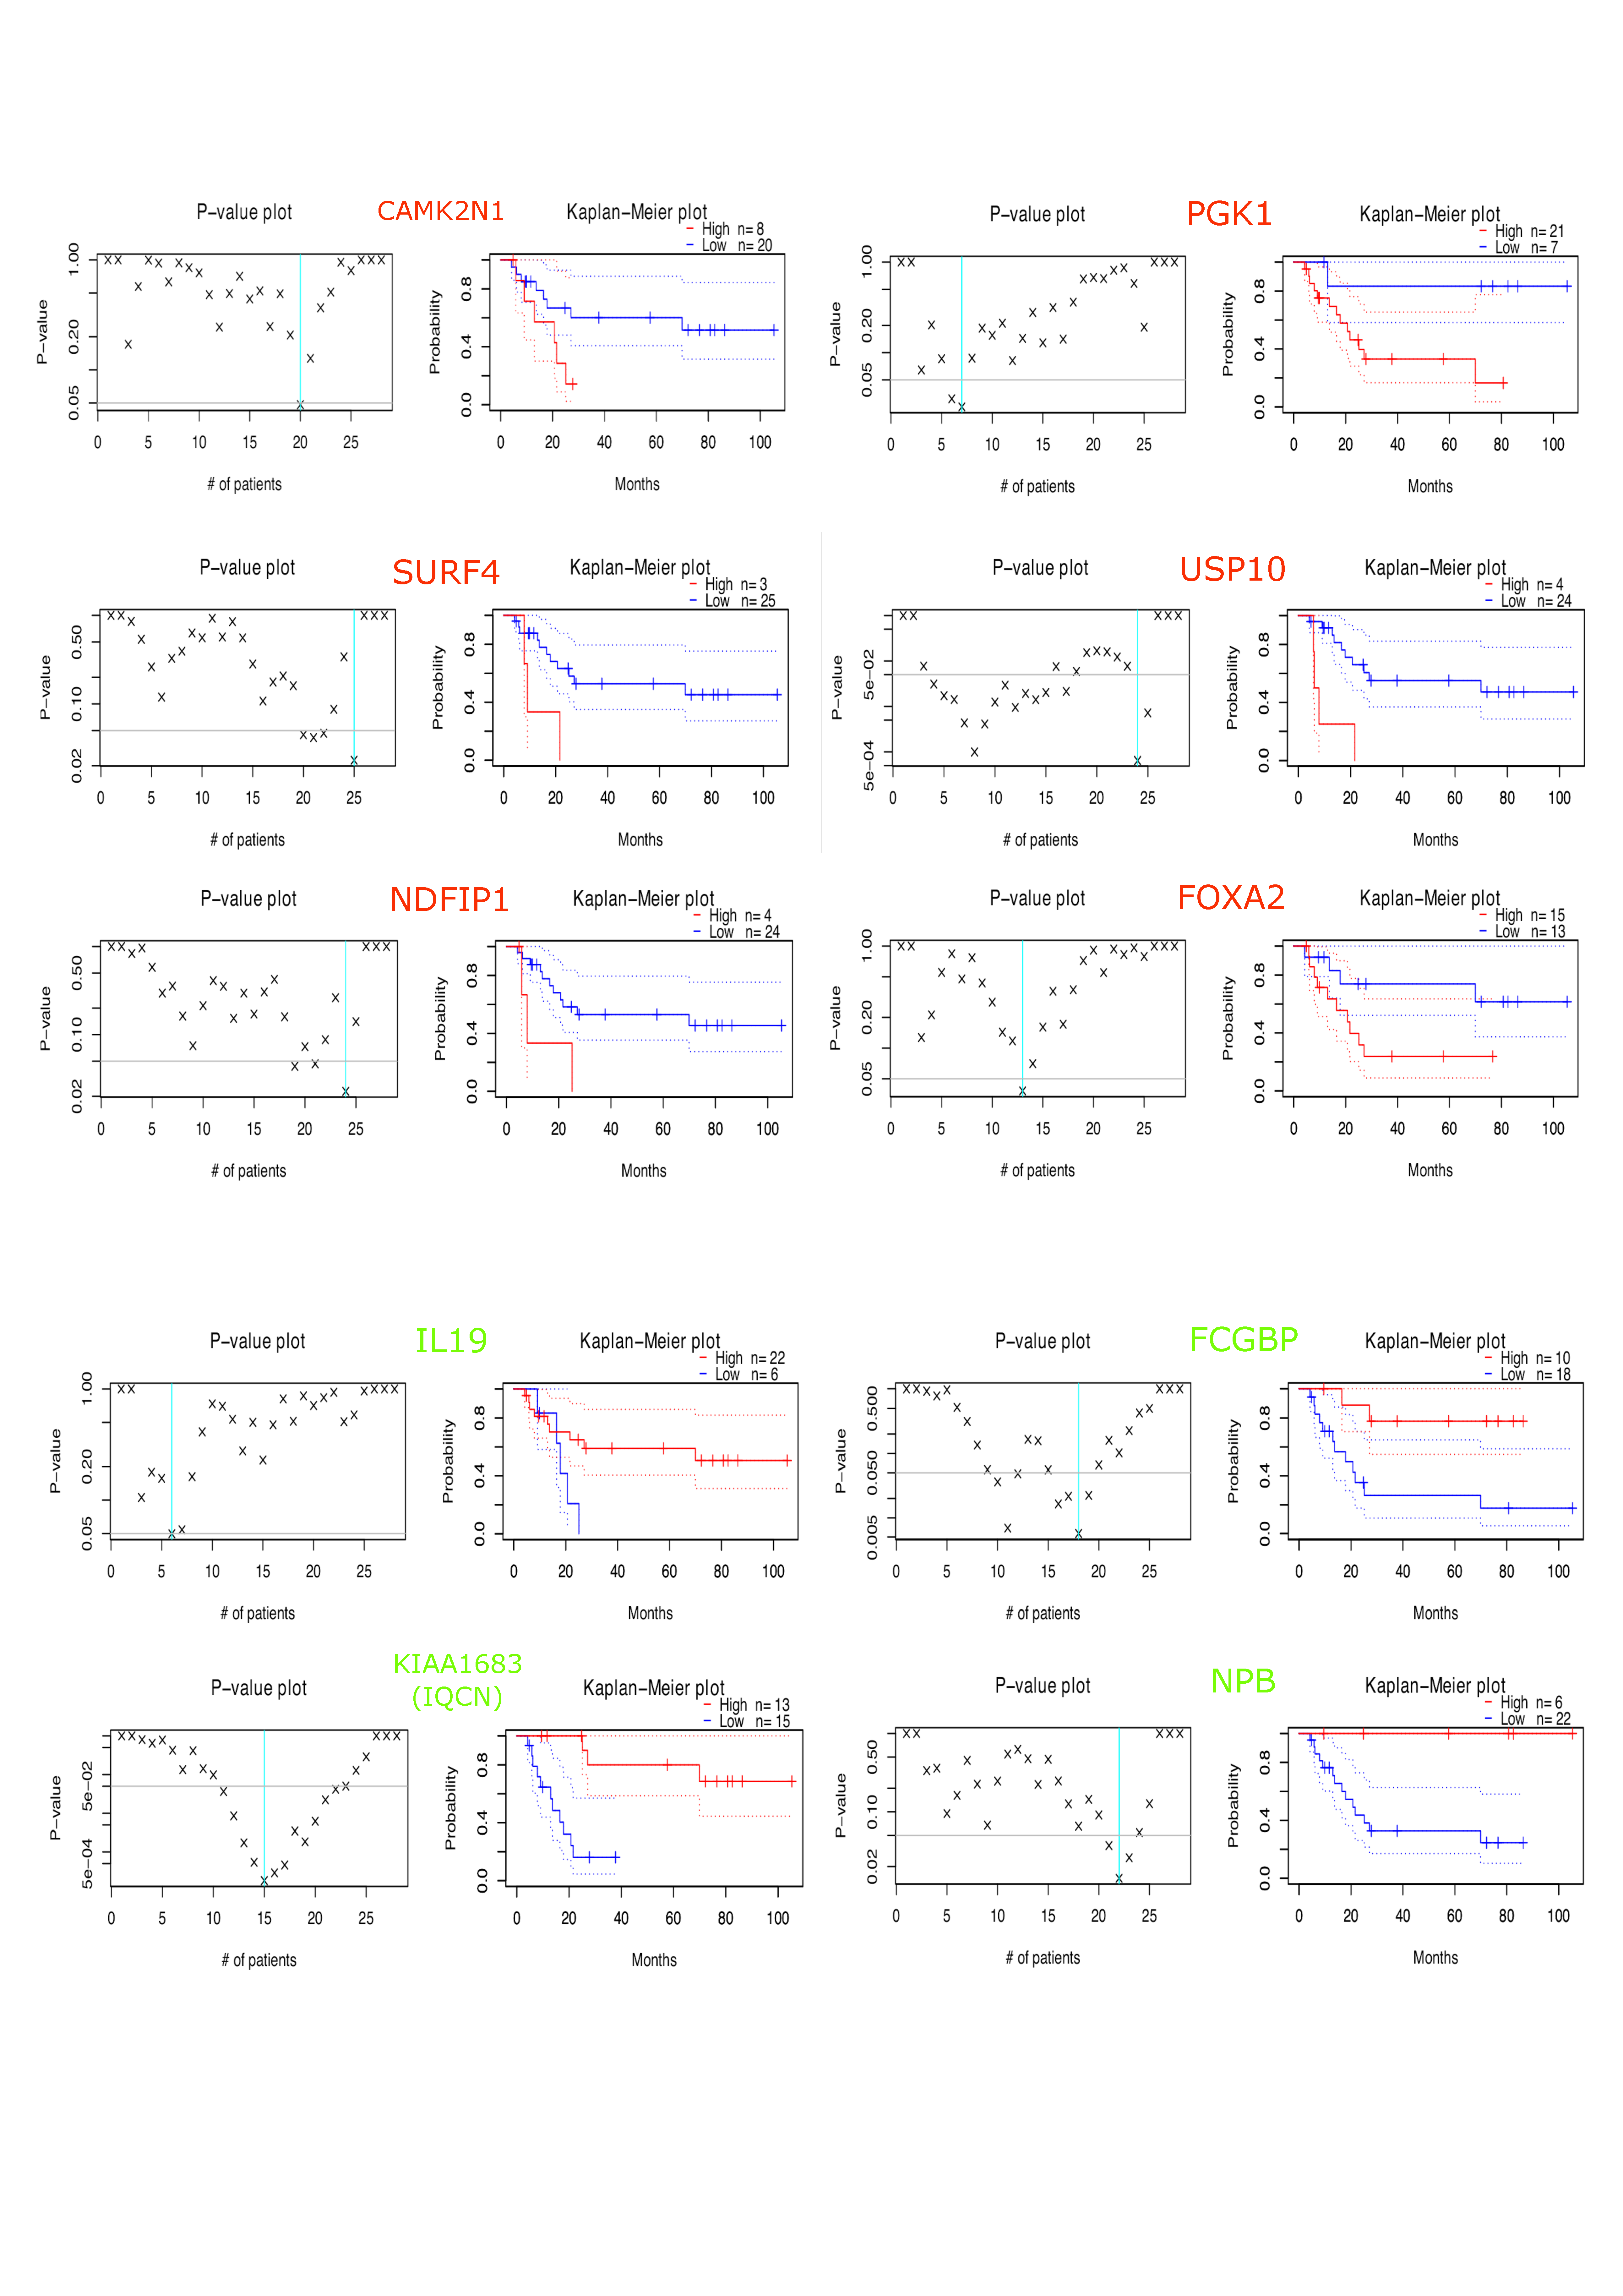
\includegraphics[width=14cm]{Answer_2-2.pdf}
\caption{GSE2837 query results from PrognoScan: Kaplan-Meier plots of 10 genes (the cutoff of \textcolor{red}{high risk} and \textcolor{blue}{low risk} groups, which is derived from cumulative P-value plots). The poor prognostic genes are marked as \textcolor{red}{red}; the better prognostic genes are marked as \textcolor{green}{green}.}
\label{figure:fig_GSE2837}
\end{figure}
\clearpage
\end{MyColorPar}

\subsection*{2-3}
Could the authors summarize the elements of the workflow that could be used on any database independently from TCGA?


\begin{MyColorPar}{blue}
Answer

We appreciate the reviewer for the critical comments and thank for your agreement of our workflow in the field of cancer research.

%how to apply or modify the R scripts to use on other datasets
%\begin{itemize} %summarize the elements of the workflow
\begin{outline}
The data from TCGA database or other databases could be applied by this workflow, since modification of the R script is necessary to adapt the difference structure among datasets (e.x. data schema, table size, definition of features, number of features and their location on the table column).\\
In short, the elements of the workflow with the \{codes\} shows:\\
(please also see Figure \ref{fig:workflow})
\1 $[\# step 1 (main)]$
\{main\_marginSFP\_HNSCC.R\}
        \2 dataset retrieval from TCGA GDC data portal (in GDAC format)
%\1 $[\# step 1]$
    \2 \{TCGA\_HNSCC\_marginSFP.R\}
        \3 \underline{raw data cleaning}
        \3 \underline{data transformation and merge}
        \3 \underline{dichotomization of clinical features}
%     \item Using a serial cut from 30\% to 70\% percentile of the cohort, it could find the least P-value cutoff of the Kaplan-Meier analysis for each gene expression.
        \3 survival analysis
            \4 cut off finder by \{cutofFinder\_func\_HNSCC.R\}
%     \item The R script program could automatically scan protein-coding genes and generate the Kaplan-Meier plots and Cox's univariate/multivariate tables.
            \4 Cox modelling
\1 $[\# step 2]$
\{analysis\_export.R\}
    \2 analysis of the tables generated from \# step 1
    \2 candidate selection
%    \item Our analysis could discover the pronounced biomarkers, which impact HNSCC's survival under the stringent Bonferroni adjustment.
\1 (remark: only the \underline{underlined} portion in \{TCGA\_HNSCC\_marginSFP.R\} should be re-coded aggressively)
\end{outline}

%\begin{outline}
%\linebreak

%\1 $[\# step 1]$
%\{TCGA\_HNSCC\_marginSFP.R\}
%    \2 raw data cleaning
%    \2 data transformation and merge
%    \2 clinical features
%\end{itemize}
%\end{outline}


%to generalize the utility of our workflow:
%R scripts could be re-coded and applied to start a new analysis of dataset.
% *** R 的特色 邊分析解讀,一邊 coding
%Currently, less HNSCC dataset is available worldwide (Indian?) => 
%能否套用在別的 database,可以,需要標準化(fpkm or RSEM)
%It made the messenger \acrshort{rnaseq} matrix with log2 transformed for the downstream analysis, as described in their reference\cite{RSEM2016}.?)
Moreover, we are planning to extend this workflow applied on other studies, such as TCGA CRC (colorectal cancer), TCGA LUAD (lung adenocarcinoma), or TCGA BRCA (breast cancer).
Then it is possible to introduce the Rstudio Shiny app (https://shiny.rstudio.com) as a web application of the "pvalueTex" packaged with our workflow in the future.

\begin{figure}
    \centering
    \includegraphics[width=14cm]{Figure_1_manuscript_workflow_modify.pdf}
    \caption{A workflow of \acrshort{hnscc} biomarker discovery, step 1 (blue line: main procedure) and step 2 (orange line: analysis export). The portion of "data process/cleaning"(red rectangled) should be modified aggressively according to different sources of databases, e.x. The NCI's TCGA Genomic Data Commons (GDC) porting to Broad Firehose, or other databases.}
    \label{fig:workflow}
\end{figure}
%(other cancer types in the TCGA database). 
%TCGA HNSCC -> TCGA CRC, TCGA LUAD, TCGA BRCA cohorts -> GEO or other uploaded cancer cohort

% workflow from the manuscript ##########
%The number of protein-coding genes was suggested as 20,500\cite{Clamp2007}. The \acrshort{gdc} Data Portal provided \acrshort{tcga} data has been harmonized and re-aligned \acrlong{rnaseq} data against an official reference genome build (\acrlong{grch38}, \acrshort{grch38}). \acrshort{rnaseq} expression level read counts produced by Illumina HiSeq have been normalized using the \acrfull{fpkm} method, as described in reference\cite{FPKM2017}.
%The \acrshort{rnaseq} preprocessor of Broad \acrshort{gdac} picked the \acrfull{rsem} value from Illumina HiSeq/GA2 messenger \acrshort{rnaseq} level\_3 (v2) dataset of \acrshort{nci} \acrshort{gdc}. It made the messenger \acrshort{rnaseq} matrix with log2 transformed for the downstream analysis, as described in their reference\cite{RSEM2016}.
%We utilized FirebrowseR's function call, Samples.mRNASeq(cohort = "HNSC", gene=GeneName, format="csv"), to download each \acrshort{rnaseq} data of all \acrshort{hnscc} patients and to save as 20,499 data frame files, named as "HNSCC.mRNA.Exp.[GeneName].\newline
%Fire.Rda".
%After careful investigation of the genomics dataset, the \acrshort{rnaseq} values of "\acrfull{slca}" and "\acrfull{slcb}" should be considered two distinct expression entities. We concluded that the number of protein-coding genes in the \acrshort{tcga} dataset is 20,500. We removed null expressed genes, which over 50\% of the cohort, to avoid the useless result.

%We utilized FirebrowseR's function call, Samples.Clinical(cohort = "HNSC", format="csv"), to get all 81 clinical features (including pathological data, defined by \acrshort{tcga} \acrshort{gdc} data dictionary: \acrfull{cde}\cite{CDE2019}) of all 528 \acrshort{hnscc} patients, which saved as one data frame file: "HNSCC.clinical.\linebreak
%Fire.Rda" (accessed November 2019).

%One "HNSCC.clinical.Fire.Rda" tables and 20,500 "HNSCC.mRNA.Exp.\newline
%[GeneName].Fire.Rda" tables were transposed and merged by their \newline
%\_participant\_barcode (unique patient \acrlong{id}, \acrshort{id}) to yield a data frame with 528 rows (participants) against 20,581 columns (81 clinical features as well as 20,500 protein-coding \acrshort{rnaseq} of cancer specimen).
%The clinicopathological features selected for our workflow included gender, age, clinical tumor size, clinical cervical lymph node metastases, clinical distant metastasis assessment, pathological surgical margin, and tobacco exposure with their corresponding survival data.
%The tumor size (T), cervical lymph node metastases (N), and distal metastasis status (M) were classified according to \acrfull{ajcc}\cite{Amin2017} along with \acrfull{uicc}\cite{Brierley2016} \acrshort{tnm} system for clinical staging of \acrshort{hnscc}.
% In the Eighth Edition, the AJCC has expanded the use of non-anatomic prognostic factors and biomarkers in assigning prognostic stage groups.
%%We made data clean by removing duplicated rows and columns.


%\subsection{Cutoff Finder Core Engine}
%To evaluate the effect of gene expression on the patient's survival, we introduced the stratifying of patients with Kaplan-Meier survival analysis according to each gene's low/high expression.
%Our cutofFinder\_func subroutine employs the minimum P-value approach to recognizing cutoff points in continuous gene expression measurement for patients sub-population.
%First, patients were ordered by \acrshort{rnaseq} value (RSEM) of a given gene. Next, patients were stratified at a serial cut (counted by person ranked in 30\% to 70\% percentile of the cohort; please see Figure \ref{fig:figure1} "HNSCC cohort"). The survival risk differences of the two groups were estimated by log-rank test to yield around 165 Kaplan-Meier P-values for each gene.
%Then, the optimal cutoff of \acrshort{rnaseq}, giving the minimum P-value, was selected by the cutofFinder\_func subroutine.
%This iteration method could calculate all possible cutoff of each gene expression in this cohort. At each run of cutofFinder\_func function call for an individual gene, it returned an optimal cutoff value (e.x. 0.027 for gene \acrlong{CAMK2N1}, \acrshort{CAMK2N1}). The optimal cutoff value and its correlated patient grouping size (e.x. low-expression in 262 persons vs. high-expression in 152 persons with gene \acrshort{CAMK2N1}) would be returned to the main program to allow downstream Cox survival analysis. The percentile range we applied as 30\% to 70\% was used to avoid a small grouping effect\cite{Miller1982}\cite{Mizuno2009a}.
%In case there was no significant P-value, a median expression of this gene was set as its cutpoint as usual.


%\subsection{Biomarker Selection}

%Those genes with prognostic impact, whose hazard ratio $>=1.5$ or $<=0.5$ in both Cox's univariate/multivariate model, were assigned as provisional candidates.
%Bonferroni adjusted (Kaplan-Meier) P-value was used to make a ranking of candidates for the final decision (see Figure \ref{fig:figure1}, step 2).



% we plan to extend this workflow on other TCGA cancer types
%Our strategy still has the strength to explore the more possible biomarkers from \acrshort{rnaseq} datasets in cancer research.
% second limitation:
%In line with tumor-agnostic research, we plan to explore more TCGA diseases to find common biomarkers. However, the \acrshort{gdc} provided standardized data frames that could not directly fit our workflow's scope. Before the global genes scanning process, we needed to re-format, transpose and, merge the 528 patients' clinical datasets and correlated 20,500 expressions of bio-specimen. It should be carefully curated to confirm the data integrity with the correct definition. We also plan to upgrade our plain R script at the Rstudio platform to program in the C++ language and source it in R. The high performance of C++ could speed up the cutoff finding engine in this workflow involving heavy computations\cite{Woodward2020}. Thus, it is possible to introduce the Rstudio Shiny app (https://shiny.rstudio.com) as a web application of the "pvalueTex" packaged with our workflow in the future.
\end{MyColorPar}


% #####################
\subsection*{2-4}
Please shortly explain the TCGA database in the Introduction and summarize the advantages of its use.

\begin{MyColorPar}{blue}
Answer

We appreciate the reviewer for the critical comment and modified the Introduction accordingly.

%https://www.cancer.gov/about-nci/organization/ccg/research/structural-genomics/tcga
% adopted from materials and methods

%The Cancer Genome Atlas (\acrshort{tcga}) profiled 528 \acrshort{hnscc} clinical and genomic data, which has been standardized and available at a unified data portal, \acrfull{gdc} of the \acrfull{nci}.
%\cite{SeanDavis;MartinMorgan2020}

\begin{MyColorPar}{red}

The Cancer Genome Atlas (TCGA) project\cite{Weinstein2013} is developed and supervised by the National Cancer Institute's (NCI) Center for Cancer Genomics and the National Human Genome Research Institute (NHGRI) funded by the US government since 2005.
TCGA represents a comprehensive genomics and clinic data from 84,392 patients among 33 major cancer types (data release 27.0 - October 29, 2020, available at https://www.cancer.gov/about-nci/organization/ccg/research/structural-genomics/tcga/studied-cancers).
%The Cancer Genome Atlas (TCGA): The TCGA consortium, which is a National Institute of Health (NIH) initiative, makes publicly available molecular and clinical information for more than 33 types of human cancers including exome (variant analysis), single nucleotide polymorphism (SNP), DNA methylation, transcriptome (mRNA), microRNA (miRNA) and proteome.

TCGA and other collaborated \acrfull{gdac} generated and analyzed DNA (mutation, copy number variation, methylation, simple nucleotide polymorphism, SNP), RNA (microarray, RNA-Seq, microRNA) and protein (reverse protein phase array) data derived from biospecimen. Sample types available at TCGA are: primary solid tumors, recurrent solid tumors, blood derived normal and tumor, metastatic, and solid tissue normal. 

The NCI's Genomic Data Commons (GDC, available at https://portal.\\gdc.cancer.gov/) receives, processes, and distributes genomic, clinical, and biospecimen data from TCGA database and other cancer research programs. The clinical features has been defined by \acrshort{tcga} \acrshort{gdc} data dictionary: \acrfull{cde}\cite{CDE2019}. The \acrshort{rnaseq} expression data has been harmonized and re-aligned against an official reference genome build (\acrlong{grch38}, \acrshort{grch38}).
%The old TCGA data portal (https://tcga-data.nci.nih.gov/docs/publications/tcga/) stops updating and all TCGA data was transferred to the GDC data portal .
\acrshort{tcga}, GDC and research community offer several computational tools to the public for facilitating cancer research. %There is three categories of tools to approach the TCGA data from GDC.

GDC Data Portal (available at https://portal.gdc.cancer.gov) is the official web-based TCGA data analysis tools. Other available web-based tools has been reviewed by Zhang et al.\cite{Zhang2019b} and 
Matthieu Foll (availalbe at https://\\github.com/IARCbioinfo/awesome-TCGA).
One of \acrshort{gdac}s, the Broad TCGA Data and Analyses (Broad GDAC), provides Firehose which is a repository of the TCGA public-accessible Level 3 data and Level 4 analyses. Broad GDAC Firehose is an analytical infrastructure to provide analyses algorithms not performed by the GDC (e.x. GISTIC, MutSig2CV, correlation with clinical variables, mRNA clustering etc.). 
A web-based version of Broad GDAC Firehose is Firebrowse (available at firebrowse.org, Version: 1.1.40 , 2019\-10\-13).
%Python and UNIX bindings
%R bindings
Broad GDAC Firebrowse provides graphical tools like viewGene to explore expression levels and iCoMut to explore a mutation analysis of each TCGA disease. 

%Second, GDC data transfer tool (available at https://gdc.cancer.gov/access-data/gdc-data-transfer-tool) allows users to access the open or controlled data. %the GDC data model, data formats
% RESTful API

GDC \acrfull{api} is designed under the \acrfull{rest} architecture and provides accessibility to external users for programmatic access to the same functionality found through GDC Portals. This includes searching, viewing, submitting and downloading subsets of data files, metadata, and annotations based on specific parameters. Moreover, if restricted data is requested, a token must be provided by the user along with the API call. This token can be downloaded directly from the GDC Portals. (this paragraph was originally published and courtesy of the National Cancer Institute)
Broad GDAC Firebrowse \acrshort{rest}ful \acrshort{api} could be accessed using an R package, FirebrowseR (available at https://github.com/mariodeng/FirebrowseR)\cite{Deng2017}.

% clinical
%We utilized FirebrowseR's function call, Samples.Clinical(cohort = "HNSC", format="csv"), to get all 81 clinical features (including pathological data, defined by \acrshort{tcga} \acrshort{gdc} data dictionary: \acrfull{cde}\cite{CDE2019}) of all 528 \acrshort{hnscc} patient.

%In summarize the advantages of its use.
In summary, the advantages of applying the TCGA data for cancer research includes:
\begin{outline}
\1  To the best of our knowledge, TCGA database is the largest collection (cancer types and cohort size) of comprehensive genomics with survival data available in the field of cancer research so far. The whole-genome sequencing data has been harmonized cross all GDACs. The basic demographic data is usually available on many database. However, TCGA data has more comprehensive features, such as exposure of alcohol, asbestos, radioactive radon, tobacco smoking or cigarette, than others.
\1  TCGA has remarkable advantage for computational and life scientists who study cancer, since useful web-tools and API are ready for analysis and visualization of TCGA data. It might be getting help easily from research community for trouble-shooting.
\1  Many achievements of diagnoses, treatments and prevention with the TCGA data have already been published and keep growing.\cite{Tomczak2015}
\end{outline}

\end{MyColorPar}   % marked in red above
In our workflow, we utilize FirebrowseR in the step 1 to receive standardized genomic and clinical data frames while avoiding data re-formatting, often causing some errors. (please also see Figure \ref{fig:workflow}, different sources of databases)
%The other GDAC, the MD Anderson GDAC's MBatch (http://bioinformatics.mdanderson.org/tcgabatcheffects) is a website that enables scientists to identify and quantify the batch effects accompanying TCGA data set, currently according to hierarchical clustering and enhanced PCA plots.

% RNA-Seq
%The \acrshort{gdc} Data Portal provided \acrshort{tcga} data has been harmonized and re-aligned \acrlong{rnaseq} data against an official reference genome build (\acrlong{grch38}, \acrshort{grch38}). \acrshort{rnaseq} expression level read counts produced by Illumina HiSeq have been normalized using the \acrfull{fpkm} method, as described in reference\cite{FPKM2017}.
%The \acrshort{rnaseq} preprocessor of Broad \acrshort{gdac} picked the \acrfull{rsem} value from Illumina HiSeq/GA2 messenger \acrshort{rnaseq} level\_3 (v2) dataset of \acrshort{nci} \acrshort{gdc}. It made the messenger \acrshort{rnaseq} matrix with log2 transformed for the downstream analysis, as described in their reference\cite{RSEM2016}.


\end{MyColorPar}
\pagebreak


\subsection*{3-1}
Comments from the reviewer \#3

%Must be improved:
%Is the research design appropriate?
%Are the results clearly presented?
*** Are the conclusions supported by the results?

Only computer computing in this research to support 20 candidate biomarkers, DKK1, CAMK2N1, STC2, PGK1, SURF4, USP10, NDFIP1, FOXA2, STIP1, DKC1, as well as ZNF557, ZNF266, IL19, MYO1H, FCGBP, LOC148709, EVPLL, PNMA5, IQCN (previous name as KIAA1683), and NPB, are all heavily associated with the prognosis of OS.

There is little information provided. The authors should provide more evidence to support this article.
%  Once the authors identify TMSB4X as a target, the rest of the analysis seems fine, but their rationale for looking into TMSB4X is not strongly supported by the available data.

\begin{MyColorPar}{blue}
Answer

We appreciate the reviewer for the critical comment. We provide more evidences mentioned below, to support the prognostic impact of these candidate genes. It needs to be further validated.
According to the reviewer's comment, the Discussion was modified accordingly (marked as red).

\begin{MyColorPar}{red}

\subsubsection*{SurvExpress} % TCGA
SurvExpress\cite{Aguirre-Gamboa2013} is
% 2021/01/23 pdf x 12 from SurvExpress
web-based tools for Biomarker comparison and validation of survival gene expression data. Using their TCGA HNSCC cohort (June 2016, n=502), the survival significance (Kaplan Meier P-value) shows in 12 genes:\\ % SurvExpress 有類似的結果:
1) poor prognosis: DKK1 (0.00005), CAMK2N1 (0.000006), STC2 (0.001), PGK1 (0.01), SURF4 (0.002), USP10 (0.002), NDFIP1 (0.000008), STIP1 (0.001), DKC1 (0.01);
%CAMK2N1 (0.048214), PGK1 (0.009978), SURF4 (0.023127), USP10 (0.017768), NDFIP1 (0.022758), FOXA2 (0.001587); % FOXA2 (0.038125)
2) better prognosis: ZNF557 (0.0007), ZNF266 (0.00008), FCGBP (0.001).
%IL19 (0.049731), FCGBP (0.005658), KIAA1683 (IQCN, 0.005886), NPB (0.014177);
%17 out of 20 candidates
%?DKK1 (0.253635),
The 12 out of 20 positive and negative prognostic genes underlined is confirmed by comparable studies using SurvExpress with TCGA cohort. Please see Figure \ref{fig:fig_SurvExpress}.

% red or green is NOT by expression level
\begin{figure}
\raggedleft
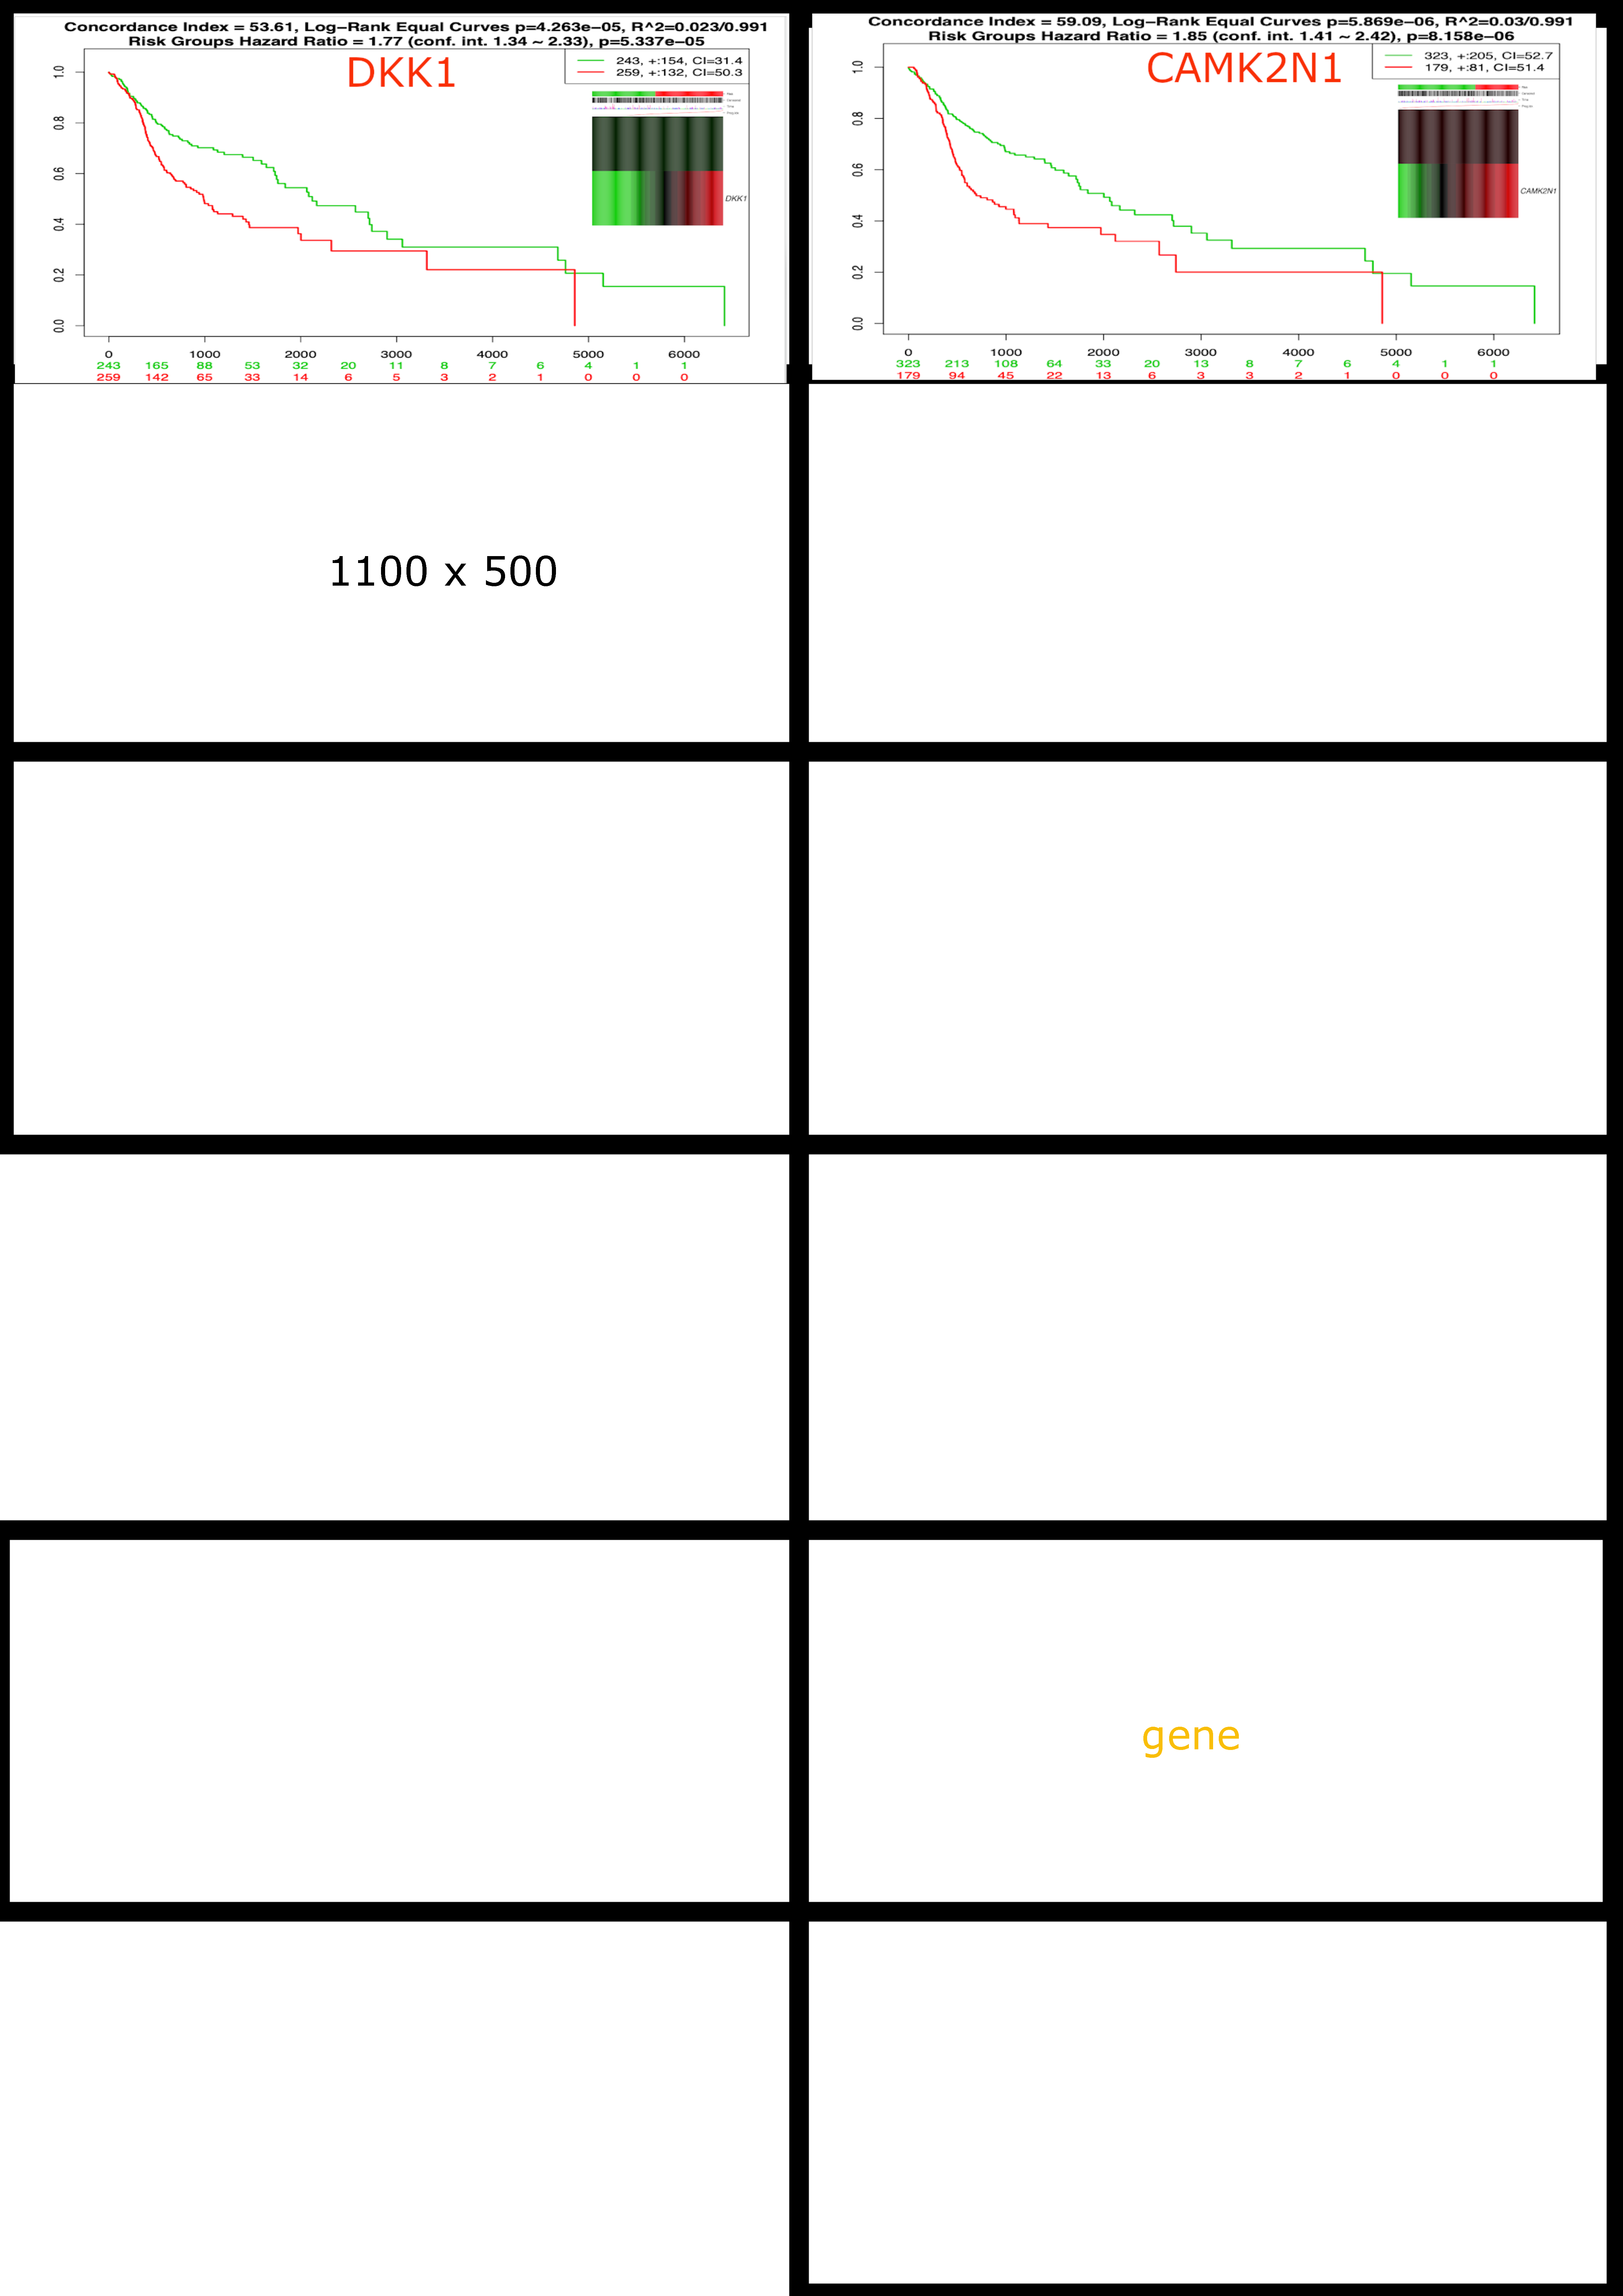
\includegraphics[width=14cm]{Answer_3-1.pdf}
\caption{The query results from SurvExpress: Kaplan-Meier plots of 12 genes (the cutoff of \textcolor{red}{high risk} and \textcolor{green}{low risk} groups, which is derived from risk groups optimization. %cumulative P-value plots).
Inset color scale shows risk groups (\textcolor{red}{high}/\textcolor{green}{low}) and corresponded RNA expression in \textcolor{red}{high}/\textcolor{green}{low}.
Thus, the poor prognostic genes are marked as \textcolor{red}{red}; the better prognostic genes are marked as \textcolor{orange}{orange}.}
\label{fig:fig_SurvExpress}
\end{figure}
\clearpage

% % SurvExpress 沒有類似的結果是因為:
Nevertheless, the survival prediction could not be found in FOXA2, IL19, MYO1H, LOC148709, EVPLL, PNMA5, IQCN, KIAA1683, NPB using SurvExpress. 
Our workflow has advantage to find an optimal cutpoint of those \acrshort{rna} expression data to maximize candidate mining coverage.
%因為 cutoff 不適當,這也就是我們 p-value Tex 的設計目的與強項

 
\subsubsection{HPA} still TCGA's RNA-Seq
The Human Protein Atlas project (HPA) Proteome analysis is based on26941 antibodies targeting 17165 unique proteins. The HPA's Pathology Atlas makes analysis of each protein in patients, using immunohistochemistry (IHC) analysis based on tissue microarrays (TMAs) adopted from TCGA. Kaplan-Meier survival analyses are based on RNA-Seq expression levels of human genes in HNSCC tissue and the clinical outcome.
All transcriptomics data has been retrieved from the Cancer Genome Atlas and all proteomics data has been generated in-house using the same antibodies.
Our candidates (DKK1, CAMK2N1, STC2, PGK1, SURF4, USP10, NDFIP1, STIP1, DKC1) are also on the list of unfavorable prognostic genes for HNSCC from \acrfull{hpa} (available at https://www.proteinatlas.org/humanproteome/pathology/head+and+neck+cancer, Version: 20.0 updated: 2020\-11\-19). The ZNF557, ZNF266, and FCGBP are on the list of favorable prognostic genes as well.
Moreover, overexpression of ubiquitin specific peptidase 10 (USP10), one of autophagy related genes, has poor prognostic impact on HNSCC, which has been proved at mRNA and protein level.\cite{Ren2020}
% 13 ARGs (GABARAPL1, ITGA3, USP10, ST13, MAPK9, PRKN, FADD, IKBKB, ITPR1, TP73, MAP2K7, CDKN2A, and EEF2K) with prognostic value were identified in HNSCC patients
found at Human Protein Atlas dataset (HPA) https://www.proteinatlas.org/ENSG00000103194-USP10/pathology/head+and+neck+cancer


% Version: 3.0.2 Date: 2015/06/11 SurvNet
%Preloaded TCGA  data is also available for analysis.
%DKK1 has the P-value 1.99328e-07 of multivariable Cox proportional hazards regression model, which was reported by network-based biomarkers research tools (SurvNet, accessed at http://bioinformatics.mdanderson.org/main/SurvNet; saved as supplementary file SurvNet\_HNSCC\_result.tsv)\cite{Li2012a}. %gene regulatory or protein interaction network
% cited by 10 articles
% he P-values pi from a univariable Cox proportional hazards regression model, which quantifies how significantly the molecular profiling data of the gene correlate with the patient survival data. 
% SurvNet also calculates the mutivariable Cox P-values for each subnetwork (a group of genes) to validate their clinical utility.
%The network files are in a '.dot' format that can be visualized by GraphViz (http://www.graphviz.org)

\subsubsection*{GSE2837} % non-TCGA
% from Anwser2-2
%by GEO GSE2837 HNSCC dataset (PrognoScan)
We analysed GSE2837 dataset (NCBI GEO database\cite{Chung2006}, HNSCC cohort has 28 participants) from online tools: PrognoScan (availalbe at http://dna00.bio.kyutech.ac.jp/PrognoScan/)\cite{Mizuno2009a}.
%??MD Anderson (40 cases) SurvNet: https://bioinformatics.mdanderson.org/SurvNet/
%https://www.ncbi.nlm.nih.gov/geo/query/acc.cgi?acc=GSE2837 \cite{Chung2006}
The GSE2837 carries
% VUMC, VAMC, UTMDACC (1992-2005)
relapse free survival (RFS) data, instead of overall survival in TCGA dataset,
and microarray gene expression (by Affymetrix X3P chips U133\_X3P).
The survival significance (Kaplan Meier P-value) is in the following probes of 10 genes:\\
1) poor prognosis: CAMK2N1 (0.048214), PGK1 (0.009978), SURF4 (0.023127), USP10 (0.017768), NDFIP1 (0.022758), FOXA2 (0.001587); % FOXA2 (0.038125)
2) better prognosis: IL19 (0.049731), FCGBP (0.005658), KIAA1683 (IQCN, 0.005886), NPB (0.014177);
%17 out of 20 candidates
%?DKK1 (0.253635), 
Please see Figure \ref{figure:fig_GSE2837}.
Nevertheless, PrognoScan has group separation cut by a skewed manner, and the GSE2837 has far less participants than TCGA cohort.
%DKK1, CAMK2N1, STC2, PGK1, SURF4, USP10, NDFIP1, FOXA2, STIP1, DKC1;
%ZNF557, ZNF266, IL19, MYO1H, FCGBP, LOC148709, EVPLL, PNMA5, KIAA1683 (IQCN), NPB
%Those 11 genes achieve similar positive and negative prognostic effect comparable with our proposed candidate genes. 
The 10 out of 20 positive and negative prognostic genes underlined is confirmed by comparable studies using GSE2837 dataset other than TCGA cohort.



\subsubsection*{Review articles}
After discovery by our workflow, we performed the literature review by Embase/Pubmed  to find the evidence of suggested 7 biomarkers in cancer research.
%Embase searching; %https://www.ncbi.nlm.nih.gov/research/pubtator/?view=docsum&query=CAMK2N1%20head%20and%20neck%20cancer
%through the PubMed searching, the remark on table 1 and table 2 presents the cancer research articles related to our candidate genes.
%PubTator Central\cite{Wei2019} is a useful Pubmed text miner

%%%%%% bad guy
The Dickkopf1 (DKK1) gene encodes a protein that was mainly involved in Wnt and other signaling pathways.
Inhibition of DKK1 in Hep-2 cells reduces their proliferation, colony formation, cell migration, and invasion in vitro\cite{Shi2014}.
Pang et al\cite{Pang2018} demonstrated that upregulation of DKK1 in SBC-3 cells (human small cell lung cancer) enhanced their proliferation, colony formation, cell migration, and invasion in vitro, as well as bone metastasis in vivo. 
Increased DKK1 levels in HNSCC tissues correlated with elevated VEGF-C and beta-catenin\cite{Shi2014}.
DKK1 expression was significantly associated with smoking, alcohol abuse, sex, human papillomavirus status\cite{Chakraborty2020}, tumor site, tumor invasion, and pathologic stage in HNSCC patients.\cite{Gao2018}.
The mRNA expression of DKK1 and DKK3 was elevated in human papillomavirus (HPV)-negative HNSCC\cite{Hu2020}. Overexpression of DKK1 indicated adverse OS in bladder urothelial carcinoma (BLCA), HNSCC\cite{Chakraborty2020}\cite{Hu2020}, and pancreatic adenocarcinoma (PAAD)\cite{Wei2020}. %Moreover, DKK1 is increased in HPV\+ HNSCC leading to the worst prognosis of the patients. 
%\cite{Shi2014}\cite{Gao2018}\cite{Chakraborty2020}(non-TCGA)\cite{Hu2020}\cite{Wei2020}
%until 2020 1. Wei, R. et al. Analyzing the prognostic value of DKK1 expression in human cancers based on bioinformatics. Ann. Transl. Med. 8, 552 (2020).\cite{Wei2020}
%using http://gepia2.cancer-pku.cn/detail.php?gene=DKK1 => \cite{Tang2019}
%GEPIA is a commonly used interactive website that plots expression profiles of given genes (from TCGA database)
%The analysis of prognosis was conducted by using the UALCAN, Gene Expression Profiling Interactive Analysis (GEPIA2)\cite{Tang2019}, and DriverDBv3 databases.


%STC2:
The miR-381 suppresses cell proliferation, migration and invasion in HNSCC SCC-4 cell line through targeting stanniocalcin 2 (STC2), and participates in HNSCC development probably via the FAK/PI3K/Akt/mTOR signaling pathway.\cite{Ma2020}

Phosphoglycerate kinase 1 (PGK1 or PGK-1), one of an glycolysis enzyme, is responsive in cisplatin-resistant HNSCC cell line (H-1R). The resistance is associated with up-regulated expression of ATP-binding cassette transporter genes (MDR1, MRP1, and MRP2), CD55, and PGK1 and down-regulated expression of Caveolin 1\cite{Nakamura2005}.

Surfeit gene 4 (SURF4): patients with tumors (such as glioma, breast cancer, lymphoma , pancreatic cancer, adrenocortical carcinoma, and sarcoma%; not HNSCC
) exhibiting high SURF4 expression had significantly shorter overall survival than low SURF4 expression. SURF4 has the potential for inducing cellular transformation and cell migration in vitro and has increased tumor growth ability in vivo\cite{Kim2018a}.
%NIH/3T3 cells (Mus musculus, mouse), 293T cell
%Loss of contact inhibition leads to phenotypic changes and promotes foci formation in vitro
%http://www.canevolve.org/AnalysisResults/AnalysisResults.html
%web-based tools survival (not TCGA?)

Ubiquitin specific peptidase 10 (USP10), one of autophagy-related genes (ARGs) may serve as a prognostic biomarker and target for in various human cancers, including epithelial ovarian cancer, colorectal cancer, and HNSCC\cite{Ren2020}.
Functional annotation - by gene set variation analysis (GSVA) and gene set enrichment analysis (GSEA) - revealed that USP10 has been significantly enriched in many critical pathways correlated with tumorigenesis of HNSCC, including the p53 pathway, IL2 STAT5 signaling, TGF beta signaling, and PI3K Ak mTOR signaling\cite{Ren2020}.
% 13 ARGs (GABARAPL1, ITGA3, USP10, ST13, MAPK9, PRKN, FADD, IKBKB, ITPR1, TP73, MAP2K7, CDKN2A, and EEF2K) with prognostic value were identified in HNSCC patients
%found at Human Protein Atlas dataset (HPA), TCGA, and (GSE6631): A total of 44 patients (22 HNSCC samples and 22 normal samples) were obtained from GSE6631. https://www.proteinatlas.org/ENSG00000103194-USP10/pathology/head+and+neck+cancer

FOXA2:
Prognostic signature integrated of DNA methylation, gene expression, and clinical information provides a prognostic prediction value for HNSCC patients 
FOXA2 is significantly associated with the poor prognosis of HNSCC through the studies of CpG-based DNA methylation and RNA expression approach\cite{Shen2017a}.
%32 HNSCC patients had both tumor and adjacent non-tumor tissue samples in TCGA cohort, which was used as the discovery set to identify differential methylation CpG sites.
%  + 0.0256 × cg03774514 FOXA2 => "+" coefficients; higher prognostic score was significantly associated with shorter survival in the training set; 
% https://www.ncbi.nlm.nih.gov/research/pubtator/?view=docsum&query=28852427
%A multi-stage screening strategy => univariate Cox regression was used to evaluate their association with overall survival in the training set, which identified 15 CpG sites with P < 0.05. Further, SIS analysis was performed to further screen out a stable probe combination. Seven of the 15 candidate CpGs were identified, including cg13495205, cg07110405, cg03774514, cg09137696, cg19655456, cg03146625, and cg21546671 (Fig. 2c, Additional file 1: Table S1), mapped to AJAP1, SHANK2, FOXA2, MT1A, ZNF570, HOXC4, and HOXB4, respectively. Using coefficients generated from Cox model, we calculated a prognostic score for each patient based on individualized values of the seven genes (Fig. 2d): prognostic score, methylation = 0.0054 × cg13495205 AJAP1  + 0.0318 × cg07110405 SHANK2 + 0.0256 × cg03774514 FOXA2  + 0.0063 × cg09137696 MT1A  + 0.0013 × cg19655456 ZNF570 − 0.0297 × cg03146625 HOXC4  − 0.0157 × cg21546671 HOXB4 .
%Association between gene expression and methylation. Left panels show correlation of a AJAP1, b SHANK2, c FOXA2, d MT1A, e ZNF570, f HOXC4, and g HOXB4 expression (X-axis) with methylation (Y-axis). Right panels show Kaplan-Meier survival plots of gene expression from the TCGA cohort. 


% non-TCGA
Stress-induced phosphoprotein 1 (STIP1, also known as HOP, P60, STI1), is increased
in the poor survival patients of ovarian cancer\cite{Chao2013}\cite{Cho2014}. T
The auto-antibody against STIP1 in serum could be a useful diagnostic biomarker for early-staged esophageal squamous cell carcinoma\cite{Xu2017}.
%STIP1 could bind to bind Hsp70 and Hsp90.


%IL-19 specifically activated an intracellular signal and induced proliferation of the cells, which indicated that IL-19 may act in an autocrine manner in oral cancer.
%IL19 in esophageal squamous cell carcinoma\cite{Hsing2013}, the effects of IL-19 on the esophageal SCC in vivo and in vitro. CE81T cells
%IL-19 may be involved in the pathogenesis of systemic inflammatory diseases. IL-19 is also involved in various inflammatory diseases such as psoriasis, asthma, and rheumatoid arthritis.
% the Chi-Mei Medical Center Institutional Review Board (IRB9705-003). n=60


%%%%%% good guy
%ZNF557 is a tumor supressor in HPV-positive HNSCC???
%Oncogenic human herpesviruses (e.x. EBV and KSHV) 
%Oncogenic human viruses are silenced through the activities of two members of the Kruppel-associated box (KRAB) domain-zinc finger protein (ZFP) (KRAB-ZFP) epigenetic silencing family, revealing a novel STAT3-KRAB-ZFP axis of virus latency.
%Epstein-Barr virus (EBV) and Kaposi’s sarcoma-associated herpesvirus (KSHV) are silenced by SZF1 and ZNF557, two members of the KRAB-ZFP repressor family\cite{Li2018c}


%ZNF266, % or ZNF16, HZF1?
%MYO1H associated mandibular prognathism\cite{Sun2018}

% IgG Fc binding protein ($Fc\gamma BP$), (Fc Fragment Of IgG Binding Protein) 
Fc fragment of IgG binding protein (($Fc\gamma BP$, FCGBP) is expressed in normal thyroid and, more significantly, it is down-regulated in papillary and follicular thyroid carcinomas.\cite{ODonovan2002}\cite{Griffith2006}
%in thyroid biopsies might help to make the difficult distinction between a thyroid follicular adenoma and a follicular carcinoma.\cite{ODonovan2002}\cite{Griffith2006}, 
%gene ID @gene@8857

%?LOC148709?, 
%EVPLL in cDNA project,
Paraneoplastic Ma 5 (PNMA5) promotes apoptosis signaling in HeLa (cervical cancer) and MCF-7 (breast cancer) cells\cite{Lee2016}

%The endogenous ligand of G protein-coupled receptors (GPR7) is IQCN (previous name as KIAA1683), and NPB (Neuropeptide B)\cite{Andreis2005}. GPR7 is associated with poor prognosis of prostate cancer\cite{Cottrell2007}. 

%calcium/calmodulin-dependent protein kinase II inhibitor (CAMK2N1) is the endogenous inhibitor of CAMK2, which is activated by an increased intracellular Ca2+ concentration.SYT12 plays a critical role in oral cancer and may be a novel therapeutic target. (PMID31598163)
%Overall survival times (as determined by Kaplan-Meier analysis) were markedly longer in patients that had elevated CAMK2N1 expression compared with patients with negative or low CAMK2N1 expression. The miR-182-5p plays a vital role in controlling OSCC cell apoptosis and proliferation by regulating CAMK2N1 expression, which was found to be reduced in OSCC. Down-regulation of miR-182-5p expression attenuated tumor growth, cell survival, and proliferation in vivo through the regulation of the AKT/ERK1/2/NF-κB signaling pathways.
%CAMK2N1 operated as a tumor suppressor gene in patients with HNSCC.
%: 26 results of cancer: ; 1 HNSCC cell line (CAL-27) all said "good guy"
%\cite{Li2018b}
%EMT genes (TCF3, CAMK2N1, EGFR, and IGFBP4) 
%x c) CCLE_RNAseq_rsem_genes_tpm_20180929.txt.gz

%NDFIP1:
%The adaptor protein Nedd4-family interacting protein 1 (NDFIP1), was reported as candidate biomarker for breast cancer\cite{Tian2020}. was both better prognosis in the overall survival (OS) and relapse free survival (RFS)
%MCF7 cells 
%Howitt et al showed that NDFIP1 knockdown results in the loss of phosphatase and tensin homolog nuclear compartmentalization, promotes cell proliferation, and alters the cell cycle
%NDFIP1 is a direct target of miR-155; MiR-155 promotes uveal melanoma cell proliferation and invasion by regulating NDFIP1 expression.
%=> good guy: Zhang et al\cite{Zhang2019a} report that miR-873 promotes Warburg effect in HCC cells by increasing glucose uptake, extracellular acidification rate (ECAR), lactate production, and ATP generation, and decreasing oxygen consumption rate (OCR) in HCC cells. Mechanistically, we show that miR-873 activates the key glycolytic proteins AKT/mTOR via targeting NDFIP1 which triggers metabolic shift. We further demonstrate that enhanced glycolysis is essential for the role of miR-873 to drive HCC progression. hepatocellular carcinoma\cite{Zhang2019a}
% MiR-873 promotes the proliferation, migration, and invasion of liver cancer cells via NDFIP1 in HEK293T cell.
%  the adaptor protein Nedd4-family interacting protein 1 (NDFIP1) plays a key role in the ubiquitination and nuclear translocation of PTEN. It represses cell proliferation of melanoma and thus acts as a tumor suppressor.(PMID: 29333944)

%DKC1 (dyskeratin) is related with HNSCC\cite{Smith2010}.
%DKC1 is the tumor suppressor gene in HNSCC
% Fanconi anemia (FA) and dyskeratosis congenita (DC) are rare inherited syndromes that cause head and neck squamous cell cancer (HNSCC).

The 9 out of 20 positive and negative prognostic genes underlined has been also suggested by published studies using TCGA cohort, in-house cohort, or experiments in vitro and in vivo.

\end{MyColorPar} % marked as red



\begin{outline} % still blue
In conclusion, 20 candidate biomarkers, DKK1, CAMK2N1, STC2, PGK1, SURF4, USP10, NDFIP1, FOXA2, STIP1, DKC1, as well as ZNF557, ZNF266, IL19, MYO1H, FCGBP, LOC148709, EVPLL, PNMA5, IQCN (previous name as KIAA1683), and NPB, are associated with the prognosis of OS in our study.
Comparison with previous publications or database analyses, 

\1 The 12 out of 20 positive and negative prognostic genes underlined is confirmed by comparable studies using SurvExpress with TCGA cohort

\1 The 12 out of 20 positive and negative prognostic genes underlined is confirmed by comparable studies using TCGA HNSCC cohort from \acrfull{hpa}. Moreover, overexpression of ubiquitin specific peptidase 10 (USP10), one of autophagy related genes, has poor prognostic impact on HNSCC, which has been proved at mRNA and protein level.\cite{Ren2020}

\1 The 10 out of 20 positive and negative prognostic genes underlined is confirmed by comparable studies using GSE2837 dataset other than TCGA cohort.

\1 The 9 out of 20 positive and negative prognostic genes underlined has been also suggested by published studies using TCGA cohort, in-house cohort, or experiments in vitro and in vivo.

\end{outline}




\end{MyColorPar}

% the end of response letter



\section{linear regression}
%Highlights
% https://quicklatex.com
\begin{flushleft}
% equation
%\begin{math}
Linear regression equation (without error term)\par
\linebreak\\[1cm]
ground truth Y:\\[0.5cm]
predicted $\hat Y$:\\[0.3cm]
$\hat Y = \beta_0 + \beta_1 X_1 + \beta_2 X_2 + \beta_3 X_3 + ... + \beta_n X_n$
\linebreak
\linebreak
input $X_1...n$
\\[0.5cm]
(predicted Y, output)
intercept
slope
independent (input) \Times
%\end{math}
\end{flushleft}

%\reftitle{References}

% Please provide either the correct journal abbreviation (e.g. according to the “List of Title Word Abbreviations” http://www.issn.org/services/online-services/access-to-the-ltwa/) or the full name of the journal.
% Citations and References in Supplementary files are permitted provided that they also appear in the reference list here. 

%\externalbibliography{yes}
%\bibliography{your_external_BibTeX_file}
\bibliographystyle{unsrt} %model1-num-names}
\bibliography{TCGA_margin_cutoff.bib}

\end{document}

